\documentclass[aspectratio=169,11pt]{beamer}
% ==========================================================================
%  KSA lecture-slide theme  =  stock beamer "Boadilla"  +  KSA colour theme
%  brand colours sampled from the official KSA symbol mark:
%    Deep Prussian Blue  #2E3192   (지성 - intellect)
%    Golden Gray         #D6CBB1   (감성 - sensibility)
%  Engine: XeLaTeX.  Usage:
%    \documentclass[aspectratio=169,11pt]{beamer}
%    \input{../../theme/ksa-theme.tex}
%  Each deck lives in its own slides/kor/<deck>/ folder together with its
%  own images; ../../figs/ is kept only as a fallback for the shared cache.
% ==========================================================================

\usepackage{fontspec}
\usepackage{amsmath,amssymb}
\usepackage{graphicx}
\graphicspath{{figs/}{./}{../../../figs/}}
\usepackage{booktabs}
\usepackage{listings}
\usepackage{varwidth}

% ---- fonts (no ctex/xeCJK on this box -> fontspec drives CJK directly) -----
\defaultfontfeatures{Ligatures=TeX}
\setmainfont{Noto Sans CJK KR}
\setsansfont{Noto Sans CJK KR}
\setmonofont{Noto Sans Mono CJK KR}[Scale=0.92]

% ---- base theme: stock Boadilla ------------------------------------------
\usetheme{Boadilla}
\usefonttheme{professionalfonts}
\setbeamertemplate{navigation symbols}{}

% ---- KSA colour theme (recolour the stock theme) --------------------------
\definecolor{ksablue}{HTML}{2E3192}
\definecolor{ksabluedk}{HTML}{20226A}
\definecolor{ksagold}{HTML}{D6CBB1}
\definecolor{ksagolddk}{HTML}{A9976B}
\definecolor{ksared}{HTML}{C0392B}
\definecolor{ksagray}{HTML}{5B5B5B}

\setbeamercolor{structure}{fg=ksablue}
\setbeamercolor{alerted text}{fg=ksared}

\setbeamercolor{palette primary}{fg=white,           bg=ksablue}
\setbeamercolor{palette secondary}{fg=white,         bg=ksablue!85!black}
\setbeamercolor{palette tertiary}{fg=white,          bg=ksabluedk}
\setbeamercolor{titlelike}{fg=ksablue}
\setbeamercolor{frametitle}{fg=ksablue,bg=}
\setbeamercolor{title}{fg=ksablue}
\setbeamercolor{author}{fg=ksagray}
\setbeamercolor{institute}{fg=ksagray}
\setbeamercolor{block title}{fg=white,bg=ksablue}
\setbeamercolor{block body}{fg=black!85,bg=ksablue!6}
\setbeamercolor{item}{fg=ksablue}
\setbeamercolor{section in toc}{fg=black!85}

\setbeamerfont{frametitle}{series=\bfseries}
\setbeamerfont{title}{series=\bfseries}

% ---- footline:  KSA mark | "Made by ..." | n / N   (matches reference) ----
\newcommand{\ksacredit}{}
\setbeamertemplate{footline}{%
  \hbox{%
    \begin{beamercolorbox}[wd=.18\paperwidth,ht=2.6ex,dp=1.5ex,leftskip=1.1em]{}%
      \raisebox{-0.35ex}{\includegraphics[height=2.0ex]{ksa-logo.png}}%
    \end{beamercolorbox}%
    \begin{beamercolorbox}[wd=.64\paperwidth,ht=2.6ex,dp=1.5ex,center]{}%
      {\scriptsize\color{ksagray}\ksacredit}%
    \end{beamercolorbox}%
    \begin{beamercolorbox}[wd=.18\paperwidth,ht=2.6ex,dp=1.5ex,rightskip=1.1em]{}%
      \hfill{\scriptsize\color{ksablue}\insertframenumber\,/\,\inserttotalframenumber}%
    \end{beamercolorbox}%
  }%
  \vskip2pt
}

% ---- section divider: stock \sectionpage, KSA-coloured -------------------
\setbeamertemplate{section page}{%
  \begingroup\centering
    {\color{ksagolddk}\rule{0.16\paperwidth}{1pt}}\par\vskip1.0em
    {\usebeamerfont{title}\color{ksablue}\insertsectionhead\par}\vskip1.0em
    {\color{ksagolddk}\rule{0.16\paperwidth}{1pt}}\par
  \endgroup
}
\AtBeginSection[]{\begin{frame}[plain,noframenumbering]\vfill\sectionpage\vfill\end{frame}}

% ---- code listings ------------------------------------------------------------
\lstdefinestyle{ksa}{%
  basicstyle=\ttfamily\scriptsize,
  keywordstyle=\color{ksablue}\bfseries,
  commentstyle=\color{ksagray}\itshape,
  stringstyle=\color{ksagolddk},
  numberstyle=\tiny\color{ksagray},
  backgroundcolor=\color{ksablue!6},
  frame=leftline, framerule=1.4pt, rulecolor=\color{ksablue},
  xleftmargin=1em, aboveskip=0.8em, belowskip=0.4em,
  showstringspaces=false, breaklines=true, language=Python,
}
\lstset{style=ksa}

% ---- handy macros -----------------------------------------------------------
\newcommand{\kb}[1]{\textbf{\color{ksablue}#1}}   % blue keyword
\newcommand{\kq}[1]{\textbf{\color{ksared}#1}}    % red key-question

\setbeamerfont{title}{series=\bfseries,size=\fontsize{24}{30}\selectfont}
\setbeamerfont{subtitle}{series=\bfseries,size=\fontsize{14}{18}\selectfont}
\setbeamerfont{author}{size=\normalsize}
\setbeamerfont{institute}{size=\small}
\graphicspath{{figs/}{../../../../assets/}}
\makeatletter
\newcommand{\markpage}[1]{\protected@write\@auxout{}{\string\newlabel{#1}{{\the\c@framenumber}{}}}\hypertarget{#1}{}}
\newcommand{\pref}[1]{\hyperlink{#1}{\textcolor{ksagolddk}{(p.\ref{#1})}}}
\makeatother

\renewcommand{\ksacredit}{Machine Learning 1 \,\textperiodcentered\, 로지스틱회귀}
\title{로지스틱회귀 (Logistic Regression)}
\subtitle{숫자 대신 확률을 예측하기}
\author{Machine Learning 1}
\institute{한국과학영재학교 (KSA)}
\date{}
\begin{document}
\begin{frame}[plain,noframenumbering]\titlepage\end{frame}

% --- 오늘의 질문
\begin{frame}{오늘의 질문}
\vfill
\centering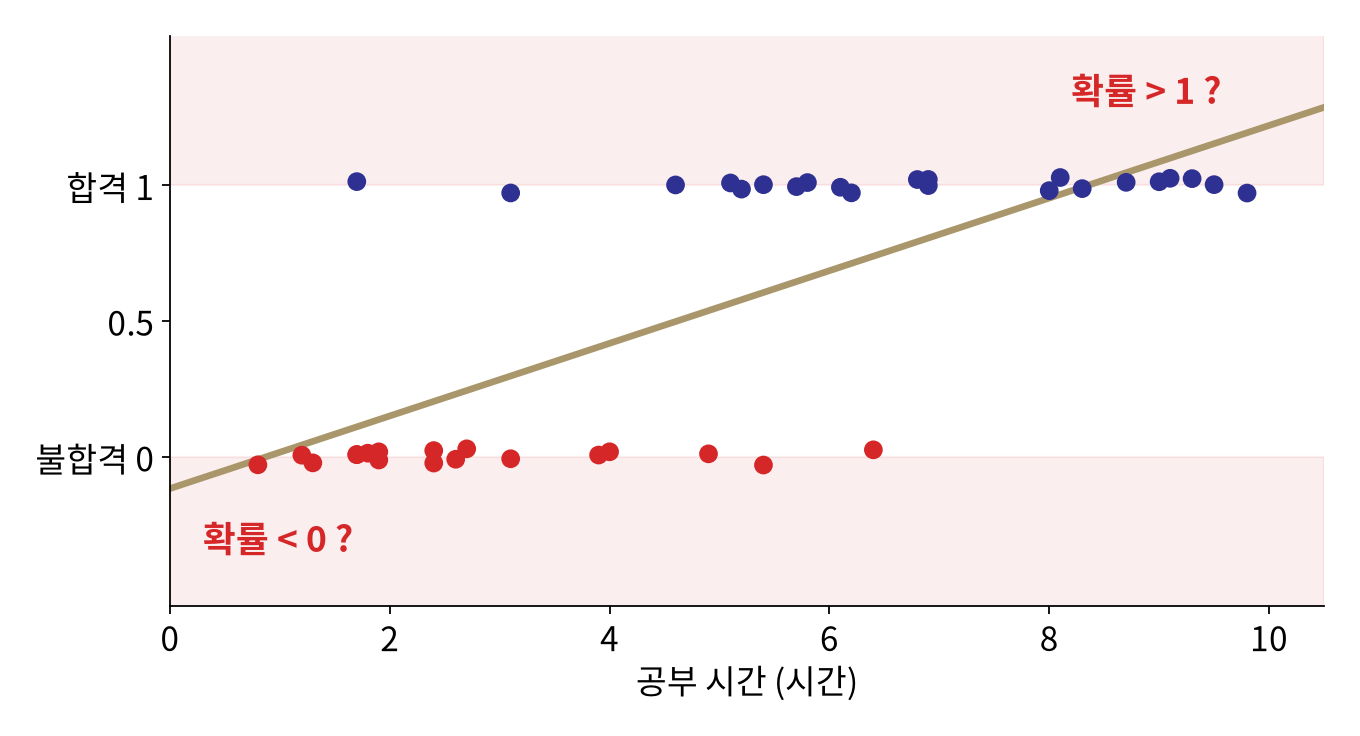
\includegraphics[width=0.6\linewidth]{logit_line.png}\par\vskip0.3em
{\large 공부 시간으로 \kb{합격(1) / 불합격(0)}을 예측하고 싶다. 선형회귀처럼 직선을 그으면?}
\vfill
\note{학생 40명의 공부 시간과 합격 여부입니다. 합격은 1, 불합격은 0입니다. 지난 시간의 선형회귀처럼 직선을 그어 보면 어떨까요? 공부를 아주 많이 하면 직선이 1을 넘어서 합격 확률 120퍼센트 같은 말이 안 되는 값이 나오고, 아주 적게 하면 0 아래로 내려갑니다. 확률을 예측하려면 출력이 항상 0과 1 사이에 있어야 합니다.}
\end{frame}

% --- 시그모이드
\begin{frame}{시그모이드: 아무 수나 0과 1 사이로}
\markpage{sigmoid}
\vfill
\begin{columns}[c]
\begin{column}{0.55\textwidth}\centering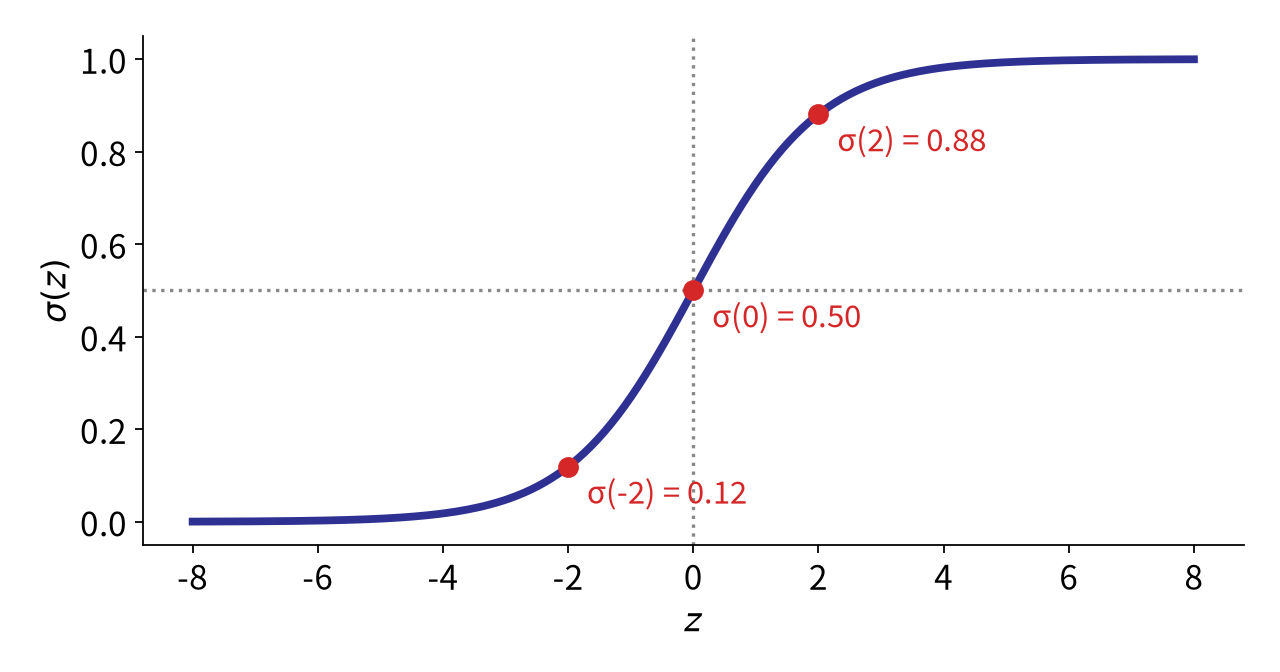
\includegraphics[width=\linewidth]{logit_sigmoid.png}\end{column}
\begin{column}{0.42\textwidth}
{\LARGE\[ \sigma(z) = \frac{1}{1 + e^{-z}} \]}\vskip0.4em
$z$ 가 크면 $\to 1$, \quad $z$ 가 작으면 $\to 0$\\[0.3em]
$z = 0$ 이면 정확히 $0.5$
\end{column}
\end{columns}
\vfill
\note{그래서 직선의 값을 시그모이드라는 함수에 한 번 통과시킵니다. 시그모이드는 어떤 수를 넣어도 0과 1 사이 값을 내놓습니다. 큰 수를 넣으면 1에 가까워지고, 작은 수를 넣으면 0에 가까워지고, 0을 넣으면 정확히 0.5가 나옵니다. 2를 넣으면 0.88, 마이너스 2를 넣으면 0.12입니다.}
\end{frame}

% --- 모델
\begin{frame}{로지스틱회귀 모델}
\vfill
\centering
{\LARGE\[ \hat y = \sigma(\underbrace{w_0 + w_1 x}_{z}) = P(\text{pass} \mid x) \]}\vskip0.6em
{\large 선형회귀의 직선 $z$ 를 그대로 쓰고, 마지막에 $\sigma$ 만 씌운다}\\[0.6em]
{\small 출력 $\hat y$ = 합격일 확률 \qquad 이름은 ``회귀''지만 하는 일은 \kb{분류}}
\vfill
\note{로지스틱회귀는 선형회귀의 직선 z를 그대로 계산하고, 마지막에 시그모이드만 씌운 모델입니다. 출력 와이햇은 x시간 공부한 학생이 합격할 확률로 읽습니다. 이름에 회귀가 들어가 있지만, 확률을 보고 합격인지 불합격인지 나누니까 실제로 하는 일은 분류입니다.}
\end{frame}

% --- 학습 결과
\begin{frame}{학습하면}
\markpage{fit}
\vfill
\centering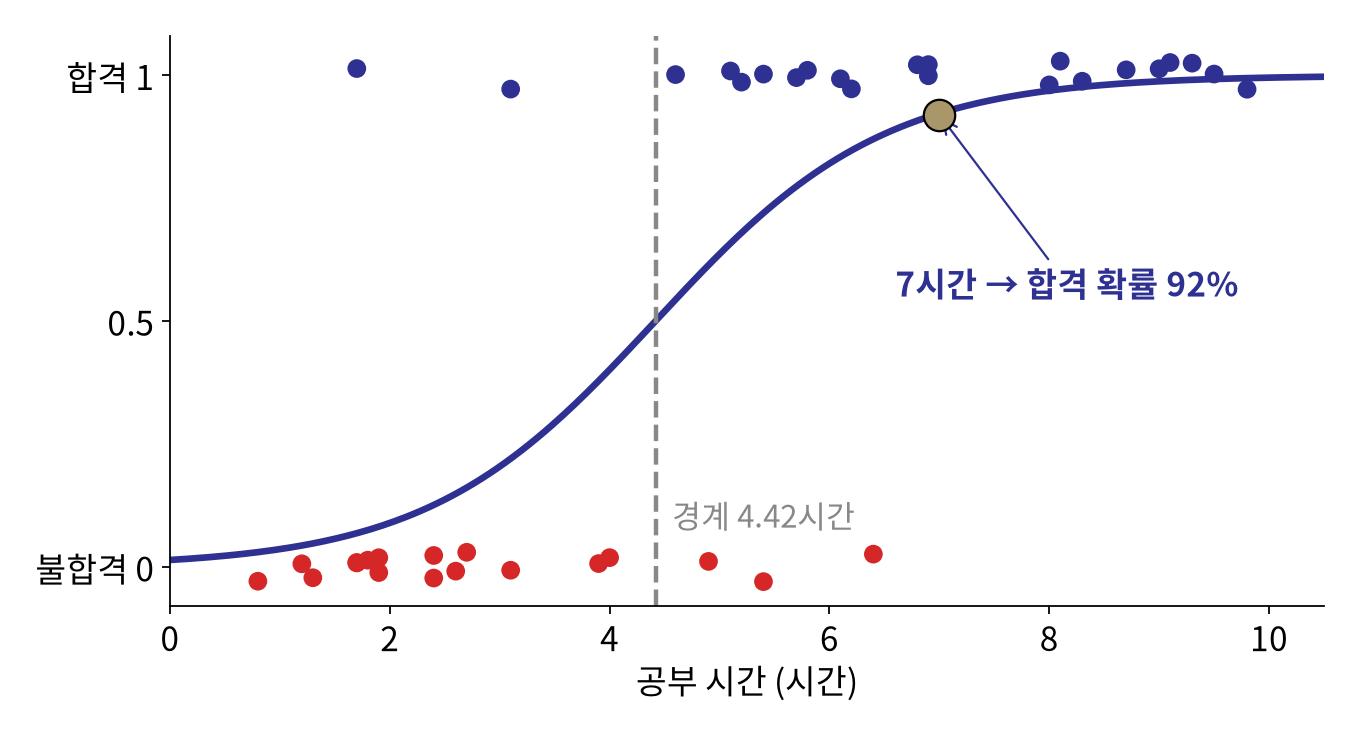
\includegraphics[width=0.6\linewidth]{logit_fit.png}\par\vskip0.3em
{\large $\hat y = \sigma(-4.24 + 0.96\,x)$ \qquad \kq{7시간 $\to$ 합격 확률 92\%}}
\vfill
\note{40명의 데이터로 학습하면 w0는 마이너스 4.24, w1은 0.96이 나옵니다. 파란 곡선이 공부 시간에 따른 합격 확률입니다. 7시간 공부한 학생의 합격 확률은 92퍼센트입니다. 회색 점선은 확률이 정확히 0.5가 되는 지점으로, 4.42시간입니다. 이보다 많이 하면 합격, 적게 하면 불합격으로 예측합니다.}
\end{frame}

% --- 결정 경계
\begin{frame}{결정 경계: $z = 0$ 인 곳}
\vfill
\centering
{\Large\[ \hat y \ge 0.5 \;\Longleftrightarrow\; z = w_0 + w_1 x \ge 0 \;\Longleftrightarrow\; x \ge -\frac{w_0}{w_1} = \frac{4.24}{0.96} \approx 4.42 \]}\vskip0.8em
{\large 시그모이드는 $z=0$ 에서 0.5 \pref{sigmoid} $\to$ \kb{경계는 직선 $z = 0$ 이 정한다}}\\[0.5em]
{\small 시그모이드는 경계의 위치를 바꾸지 않는다. 확률로 바꿔 줄 뿐}
\vfill
\note{확률이 0.5 이상이면 합격이라고 할 때, 그 경계가 어디인지 식으로 구해 봅시다. 시그모이드는 z가 0일 때 0.5니까, 와이햇이 0.5 이상인 것은 z가 0 이상인 것과 같습니다. z는 w0 더하기 w1 x이니까 x가 마이너스 w0 나누기 w1, 4.42 이상이면 됩니다. 시그모이드는 경계의 위치를 바꾸지 않고, 경계로부터 얼마나 떨어졌는지를 확률로 바꿔 줄 뿐입니다.}
\end{frame}

% --- 두 특징
\begin{frame}{특징이 둘이면: 경계는 직선}
\vfill
\centering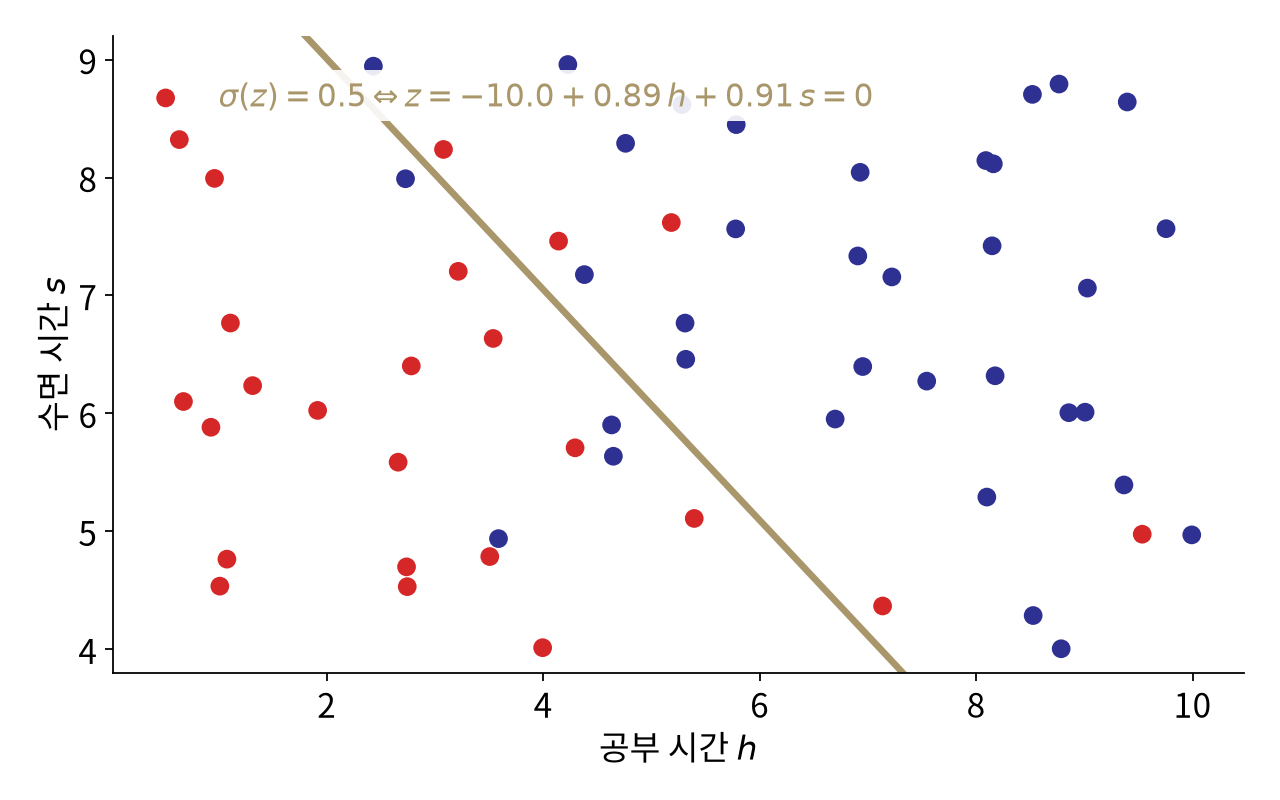
\includegraphics[width=0.5\linewidth]{logit_2d.png}\par\vskip0.2em
{\large 공부 시간 $h$ 와 수면 시간 $s$: 경계 $w_0 + w_1 h + w_2 s = 0$ 은 평면 위의 \kb{직선}}
\vfill
\note{특징이 두 개면 어떨까요? 공부 시간과 수면 시간으로 합격을 예측해 봅니다. 파란 점이 합격, 빨간 점이 불합격입니다. z는 w0 더하기 w1 h 더하기 w2 s이고, z가 0인 곳이 경계니까 이건 평면 위의 직선입니다. 공부를 덜 했어도 잠을 충분히 잤으면 합격 쪽에 들어갈 수 있다는 뜻입니다. 특징이 더 많아지면 경계는 평면, 초평면이 되지만 여전히 곧습니다. 그래서 로지스틱회귀를 선형 분류기라고 부릅니다.}
\end{frame}

% --- 오즈
\begin{frame}{$w_1$ 을 읽는 법: 오즈}
\vfill
\centering
{\Large\[ z = \ln \frac{p}{1-p} \qquad \text{odds} = \frac{p}{1-p} = \frac{\text{합격 확률}}{\text{불합격 확률}} \]}\vskip0.6em
{\large 공부를 1시간 더 하면 $z$ 가 $w_1$ 만큼 커진다 $\to$ 오즈가 $e^{w_1} = e^{0.96} \approx$ \kq{2.61배}}\\[0.6em]
{\small 예: 합격 확률 50\% (오즈 1) $\to$ 1시간 더 하면 오즈 2.61, 확률 $2.61/3.61 \approx 72\%$}
\vfill
\note{w1은 어떻게 해석할까요? 시그모이드를 거꾸로 풀면 z는 로그 오즈가 됩니다. 오즈는 합격 확률을 불합격 확률로 나눈 값으로, 내기에서 몇 대 몇이라고 할 때 쓰는 그 비율입니다. 공부를 1시간 더 하면 z가 w1만큼 커지니까, 오즈는 e의 w1제곱, 약 2.61배가 됩니다. 예를 들어 합격 확률이 반반이던 학생이 1시간 더 하면 오즈가 1에서 2.61로, 확률로는 약 72퍼센트가 됩니다. 의학이나 사회과학 논문에서 로지스틱회귀를 이렇게 해석합니다.}
\end{frame}

% --- 손실
\begin{frame}{손실: 교차 엔트로피}
\vfill
\centering
{\Large\[ J(\boldsymbol w) = -\frac{1}{m}\sum_{i=1}^{m} \Big[\, y^{(i)} \ln \hat y^{(i)} + (1-y^{(i)}) \ln (1-\hat y^{(i)}) \,\Big] \]}\vskip0.6em
{\large 정답 쪽에 준 확률에 $-\ln$ \quad (교차 엔트로피 차시의 ``칩 걸기'')}\\[0.5em]
{\small 오차 제곱(MSE)을 쓰면 확신하고 틀렸을 때 기울기가 사라진다 $\to$ 교차 엔트로피를 쓴다}
\vfill
\note{학습에는 교차 엔트로피를 손실로 씁니다. 정답이 1이면 1일 확률에, 정답이 0이면 0일 확률에 마이너스 로그를 씌운 값을 평균 냅니다. 교차 엔트로피 시간에 본 칩 걸기 벌점 그대로입니다. 선형회귀처럼 오차 제곱을 쓰면, 확신하고 틀린 학생에서 기울기가 0에 가까워져 학습이 멈춘다는 것도 그 시간에 봤습니다.}
\end{frame}

% --- 기울기
\begin{frame}{기울기: 선형회귀와 똑같은 모양}
\markpage{grad}
\vfill
\centering
{\Large\[ \frac{\partial J}{\partial w_j} = \frac{1}{m}\sum_{i=1}^{m} \big(\hat y^{(i)} - y^{(i)}\big)\, x_j^{(i)} \]}\vskip0.6em
{\large 선형회귀: $\hat y = z$ \qquad 로지스틱회귀: $\hat y = \sigma(z)$}\\[0.4em]
{\large \kb{``오차 $\times$ 입력의 평균''}이라는 모양은 같다 $\to$ 경사하강법 코드도 한 줄만 다르다}\\[0.6em]
{\small 시그모이드의 미분 $\hat y(1-\hat y)$ 이 교차 엔트로피의 $1/\hat y$, $1/(1-\hat y)$ 과 약분되어 생긴 결과}
\vfill
\note{놀라운 점이 하나 있습니다. 교차 엔트로피를 w로 미분하면, 오차 와이햇 빼기 y에 입력을 곱해서 평균 낸 값이 나옵니다. 선형회귀의 기울기와 모양이 똑같습니다. 다른 점은 와이햇이 직선 값이냐, 시그모이드를 씌운 값이냐 하나뿐입니다. 시그모이드의 미분이 교차 엔트로피의 분모와 약분되어서 생긴 결과입니다. 그래서 선형회귀 경사하강법 코드에서 예측하는 줄 하나만 바꾸면 로지스틱회귀가 됩니다. 실습에서 직접 해 봅니다.}
\end{frame}

% --- 임계값
\begin{frame}{0.5 만이 답은 아니다: 임계값}
\vfill
\centering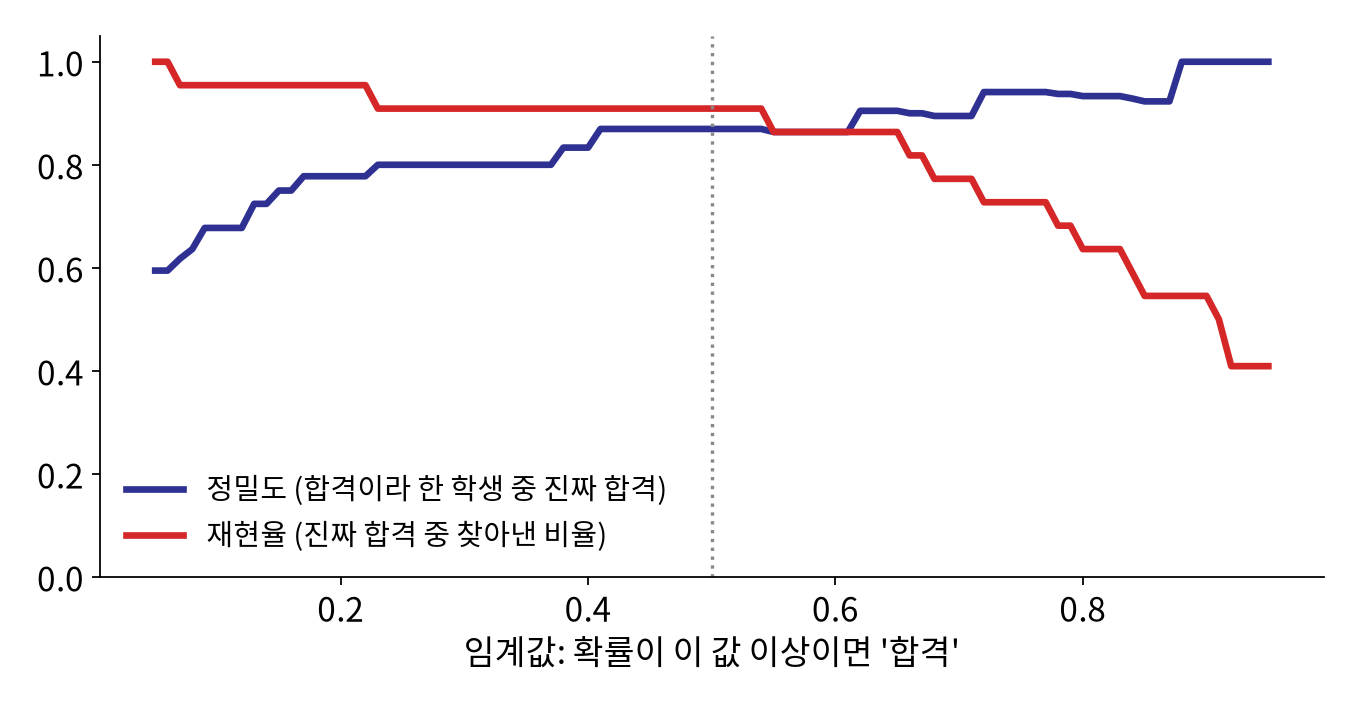
\includegraphics[width=0.6\linewidth]{logit_threshold.png}\par\vskip0.2em
{\large 임계값을 올리면 \kb{정밀도} $\uparrow$ \kq{재현율} $\downarrow$ \quad 무엇을 놓치면 더 곤란한지로 정한다}
\vfill
\note{확률 0.5 이상을 합격이라고 하는 건 하나의 선택일 뿐입니다. 임계값을 올리면 확실한 학생만 합격이라고 하니까, 합격이라고 한 학생 중 진짜 합격 비율인 정밀도는 오르고, 진짜 합격생 중 찾아낸 비율인 재현율은 내려갑니다. 1주차에 본 암 진단 키트처럼, 놓치는 게 더 무서운 문제라면 임계값을 낮추고, 헛짚는 게 더 곤란하면 높입니다. 임계값을 모두 훑어서 정밀도와 재현율을 한 그림에 그린 것이 PR 곡선이고, 그 아래 넓이가 PR-AUC입니다. 실습에서 그려 봅니다.}
\end{frame}

% --- 문제풀이
\begin{frame}{문제풀이}
\vfill
\begin{enumerate}
\item $\sigma(0)$ 은? $\sigma(z) = 0.9$ 이면 $z$ 는? \; ($\ln 9 \approx 2.2$)\vskip0.7em
\item 모델 $\hat y = \sigma(-6 + 1.5\,x)$. (a) 결정 경계 $x$ 는? \; (b) $x = 4$ 일 때 합격 확률은?\vskip0.7em
\item $w_1 = 0.7$ 이면 $x$ 가 1 늘 때 오즈는 몇 배? \; ($e^{0.7} \approx 2.0$)\vskip0.7em
\item 정답 $y = 1$, 예측 $\hat y = 0.8$, 입력 $x = 3$. 이 데이터 하나의 $\partial J / \partial w_1$ 은? \pref{grad}
\end{enumerate}
\vfill
\note{1번 답. 시그모이드 0은 0.5입니다. 시그모이드 z가 0.9이면 오즈가 0.9 나누기 0.1, 9이니까 z는 ln 9, 약 2.2입니다. 2번 답. 경계는 z가 0인 곳, 마이너스 6 더하기 1.5 x가 0이니 x는 4입니다. 그래서 x가 4이면 정확히 경계 위라서 확률은 0.5입니다. 3번 답. e의 0.7제곱, 약 2배입니다. 4번 답. 오차 와이햇 빼기 y는 마이너스 0.2, 여기에 x 3을 곱해서 마이너스 0.6입니다. 기울기가 음수이니 w1을 키우는 쪽으로 갑니다.}
\end{frame}

% --- 실습
\begin{frame}[fragile]{실습}
\vfill
\centering\begin{tabular}{rl}
\large 1 & 선형회귀 코드에서 한 줄 바꿔 로지스틱회귀 구현: 7시간 $\to$ 92\% 재현\\[0.5em]
\large 2 & 타이타닉 생존 예측: 성별 · 객실 등급 · 나이의 오즈 배수 읽기\\[0.5em]
\large 3 & 임계값을 바꿔 정밀도 · 재현율 보기, PR 곡선과 PR-AUC
\end{tabular}\vskip1em
Titanic (승객 891명, seaborn-data) \\[0.4em]\href{https://colab.research.google.com/github/SuminHan/book-ml/blob/main/slides/v2/ml1/week02/logistic_regression/lab/logistic_regression.ipynb}{\textcolor{ksagolddk}{▶ Colab에서 실습 노트북 열기}}
\vfill
\note{실습은 세 부분입니다. 첫째, 지난 시간의 선형회귀 경사하강법 코드에서 예측 줄 하나를 시그모이드로 바꿔 로지스틱회귀를 만들고, 7시간 92퍼센트를 재현합니다. 둘째, 타이타닉 승객 891명의 생존 여부를 성별, 객실 등급, 나이로 예측하고, 각 특징의 오즈 배수를 읽어 봅니다. 셋째, 임계값을 바꿔 가며 정밀도와 재현율이 어떻게 바뀌는지 보고 PR 곡선을 그립니다.}
\end{frame}

% --- 정리
\begin{frame}{정리}
\vfill
\centering\large\begin{tabular}{l}
모델 \quad $\hat y = \sigma(w_0 + w_1 x)$ = 1일 확률\\[0.5em]
결정 경계 \quad $z = 0$ (특징이 여럿이어도 곧은 경계)\\[0.5em]
해석 \quad $x$ 가 1 늘면 오즈가 $e^{w_1}$ 배\\[0.5em]
학습 \quad 교차 엔트로피 + 경사하강법 (기울기는 선형회귀와 같은 모양)\\[0.5em]
판정 \quad 임계값은 정밀도 · 재현율을 보고 정한다
\end{tabular}
\vfill
\note{정리합니다. 로지스틱회귀는 직선에 시그모이드를 씌워 1일 확률을 내는 모델입니다. 결정 경계는 z가 0인 곳이고, 특징이 여럿이어도 곧은 경계입니다. w1은 x가 1 늘 때 오즈가 e의 w1제곱 배가 된다고 읽습니다. 학습은 교차 엔트로피와 경사하강법으로 하고, 기울기는 선형회귀와 같은 모양입니다. 마지막으로 0.5라는 임계값은 정밀도와 재현율을 보고 문제에 맞게 정합니다.}
\end{frame}
\end{document}
